%%%%%%%%%%%%%%%%%%%%%%%%%%%%%%%%%%%%

\section{Experiments}

%%%%%%%%%%%%%%%%%%%%%%%%%%%%%%%%%%%%

\begin{frame}
\frametitle{Principles of experimental design}

\begin{enumerate}

\item \hl{Control:} Compare treatment of interest to a control group.

\item \hl{Randomize:} Randomly assign subjects to treatments, and randomly sample from the population whenever possible.

\item \hl{Replicate:} Within a study, replicate by collecting a sufficiently large sample. Or replicate the entire study.

\item \hl{Block:} If there are variables that are known or suspected to affect the response variable, first group subjects into \hl{blocks} based on these variables, and then randomize cases within each block to treatment groups.

\end{enumerate}

\end{frame}

%%%%%%%%%%%%%%%%%%%%%%%%%%%%%%%%%%%%

\begin{frame}
\frametitle{More on blocking}


\twocol{0.25}{0.75}
{
\begin{center}
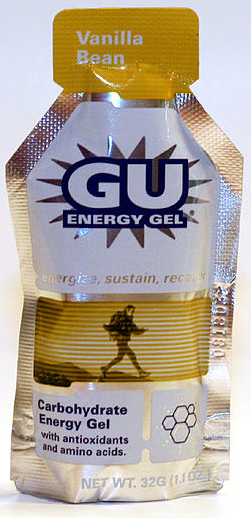
\includegraphics[width=\textwidth]{1-3_data_collection_principles/figures/gu}
\end{center}
}
{
\begin{itemize}
\item We would like to design an experiment to investigate if energy gels makes you run faster:

\pause

\begin{itemize}
\item Treatment: energy gel
\item Control: no energy gel
\end{itemize}

\pause

\item It is suspected that energy gels might affect pro and amateur athletes differently, therefore we block for pro status:

\pause

\begin{itemize}
\item Divide the sample to pro and amateur
\item Randomly assign pro athletes to treatment and control groups
\item Randomly assign amateur athletes to treatment and control groups
\item Pro/amateur status is equally represented in the resulting treatment and control groups
\end{itemize}
\end{itemize}
}

\pause

\dq{Why is this important? Can you think of other variables to block for?}

\end{frame}

%%%%%%%%%%%%%%%%%%%%%%%%%%%%%%%%%%%%

\begin{frame}
\frametitle{Practice}

\pq{A study is designed to test the effect of light level and noise level on exam performance of students. The researcher also believes that light and noise levels might have different effects on males and females, so wants to make sure both genders are equally represented in each group. Which of the below is correct?}

\begin{enumerate}[(a)]
\item There are 3 explanatory variables (light, noise, gender) and 1 response variable (exam performance)
\solnMult{There are 2 explanatory variables (light and noise), 1 blocking variable (gender), and 1 response variable (exam performance)}
\item There is 1 explanatory variable (gender) and 3 response variables (light, noise, exam performance)
\item There are 2 blocking variables (light and noise), 1 explanatory variable (gender), and 1 response variable (exam performance)
\end{enumerate}

\end{frame}

%%%%%%%%%%%%%%%%%%%%%%%%%%%%%%%%%%%%

\begin{frame}
\frametitle{Difference between blocking and explanatory variables}

\begin{itemize}

\item Factors are conditions we can impose on the experimental units.

\item Blocking variables are characteristics that the experimental units come with, that we would like to control for.

\item Blocking is like stratifying, except used in experimental settings when randomly assigning, as opposed to when sampling.

\end{itemize}

\end{frame}

%%%%%%%%%%%%%%%%%%%%%%%%%%%%%%%%%%%%

\begin{frame}
\frametitle{More experimental design terminology...}

\begin{itemize}

\item \hl{Placebo:} fake treatment, often used as the control group for medical studies

\item \hl{Placebo effect:} experimental units showing improvement simply because they believe they are receiving a special treatment

\item \hl{Blinding:} when experimental units do not know whether they are in the control or treatment group

\item \hl{Double-blind:} when both the experimental units and the researchers who interact with the patients do not know who is in the control and who is in the treatment group

\end{itemize}

\end{frame}

%%%%%%%%%%%%%%%%%%%%%%%%%%%%%%%%%%%%

\begin{frame}
\frametitle{Practice}

\pq{What is the main difference between observational studies and experiments?}

\begin{enumerate}[(a)]
\item Experiments take place in a lab while observational studies do not need to.
\item In an observational study we only look at what happened in the past.
\solnMult{Most experiments use random assignment while observational studies do not.}
\item Observational studies are completely useless since no causal inference can be made based on their findings.
\end{enumerate}

\end{frame}

%%%%%%%%%%%%%%%%%%%%%%%%%%%%%%%%%%%%

\begin{frame}
\frametitle{Random assignment vs. random sampling}

\begin{center}
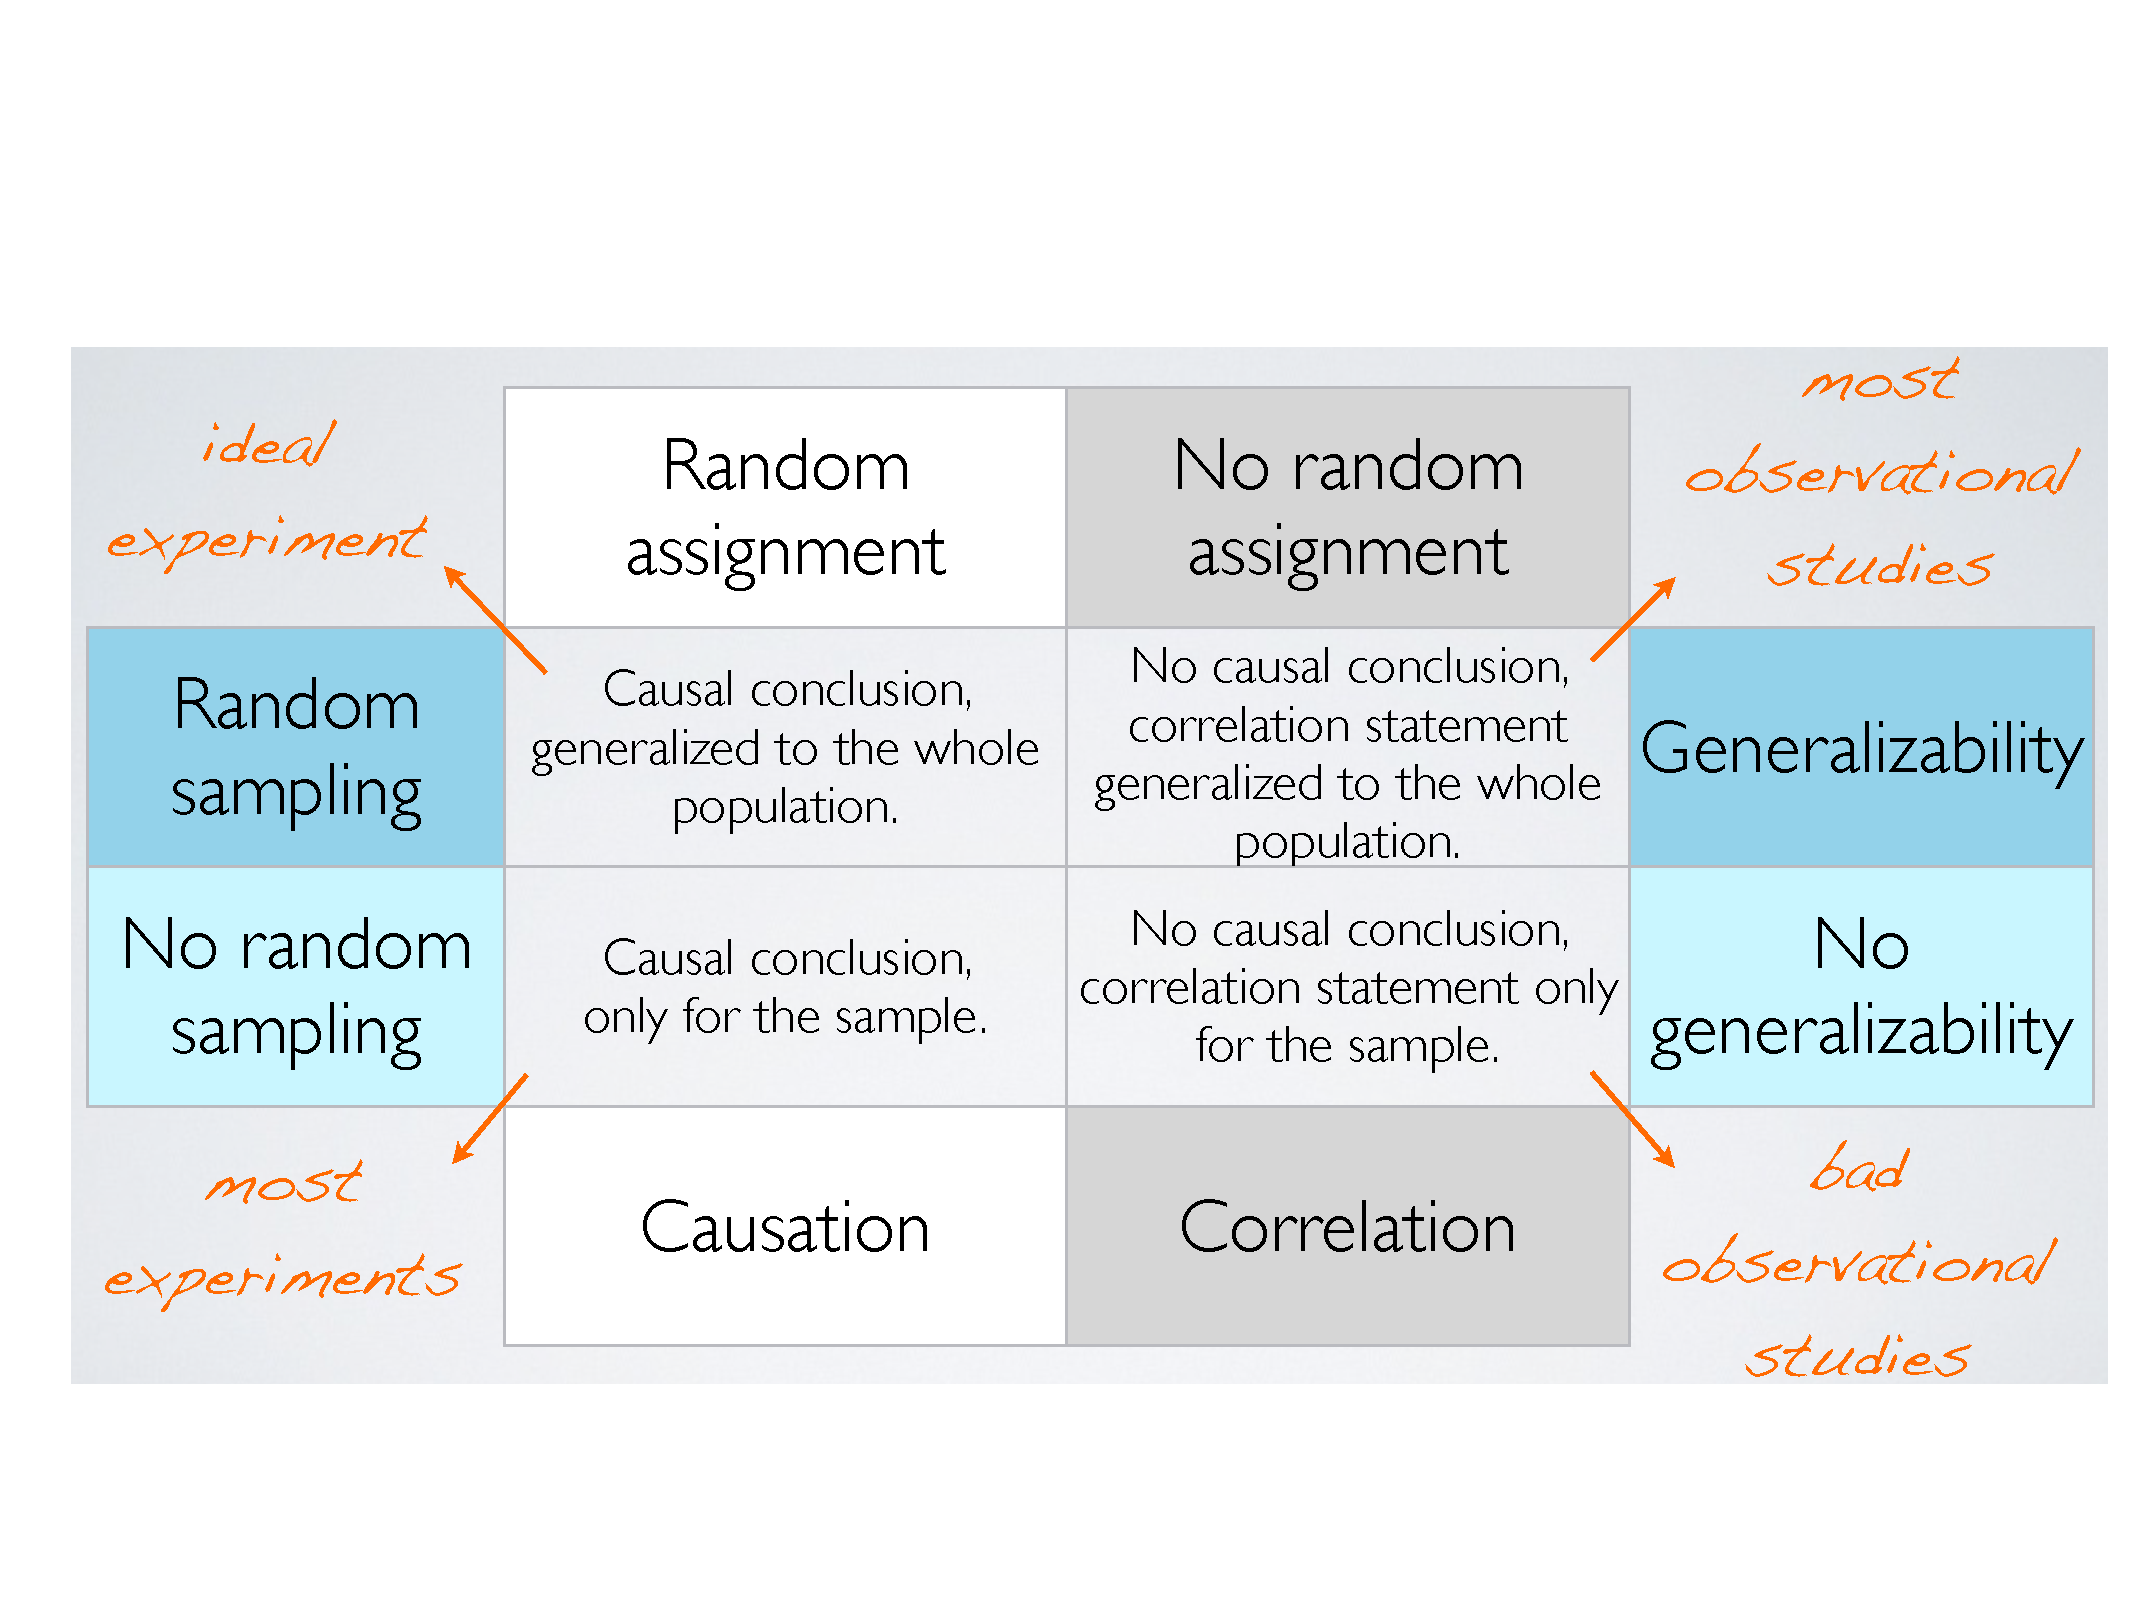
\includegraphics[width=\textwidth]{1-5_experiments/figures/random_sample_assignment}
\end{center}

\end{frame}

%%%%%%%%%%%%%%%%%%%%%%%%%%%%%%%%%%%%
